\subsection{Maximised Airspace Utilisation}

% To accommodate growing air traffic demand and integrate \gls{UAM}, airspace utilisation must be maximised efficiently and safely. 
% Two key EU-funded projects: Metropolis and Metropolis 2, have explored how structured airspace and separation management strategies can address these challenges.

The increasing demand for \gls{UAM} and the integration of \glspl{UAV} into controlled airspace present major challenges for traditional \gls{ATM}. 
To maximise the use of limited urban airspace while maintaining safety and efficiency, novel airspace design concepts and AI-driven separation management techniques are being explored.

\subsubsection{Metropolis Project: Structuring the Airspace}

The first Metropolis project investigated how different airspace structures affect capacity, complexity, safety, and efficiency in high-density urban environments. 
It introduced four airspace concepts: Full Mix, Layers, Zones, and Tubes, each offering varying levels of structure to manage \gls{UAV} traffic (Figure~\ref{airspace-concepts}):

\begin{itemize}
    \item \textbf{Full Mix:} An unstructured airspace where aircraft navigate based only on physical constraints such as terrain and weather.
    \item \textbf{Layers:} Vertically segmented bands that restrict aircraft heading directions, providing horizontal deconfliction through altitude separation.
    \item \textbf{Zones:} Airspace divided based on city layout, resembling current manned airspace practices.
    \item \textbf{Tubes:} Predefined, fixed aerial corridors that create conflict-free zones for structured traffic flow.
\end{itemize}

\begin{figure}[!ht]
    \centering
    \begin{subfigure}{.23\textwidth}
        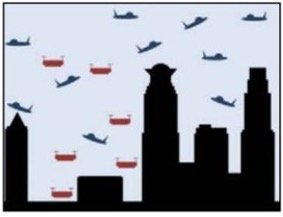
\includegraphics[width=\textwidth]{img/full-mix.jpg}
        \caption{Full-Mix}
        \label{full-mix}
    \end{subfigure}
    \begin{subfigure}{.23\textwidth}
        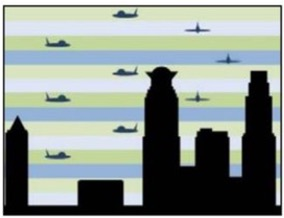
\includegraphics[width=\textwidth]{img/layers.jpg}
        \caption{Layers}
        \label{layers}
    \end{subfigure}
    \begin{subfigure}{.23\textwidth}
        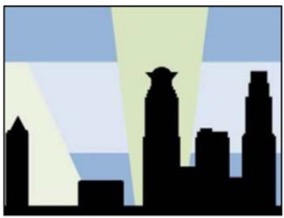
\includegraphics[width=\textwidth]{img/zones.jpg}
        \caption{Zones}
        \label{Zones}
    \end{subfigure}
    \begin{subfigure}{.23\textwidth}
        
\includegraphics[width=\textwidth]{img/tubes.jpg}
        \caption{Tubes}
        \label{tubes}
    \end{subfigure}
    \caption{Metropolis: Airspace concepts \cite{Schuchardt_2023}.}
    \label{airspace-concepts}
\end{figure}

In simulations performed by Sunil et al. \cite{Sunil_2015}, conflict resolution was handled by the \gls{MVP} algorithm in the Full Mix, Layers, and Zones concepts. 
In Zones and Tubes, A* algorithm was used to determine the shortest trajectory prior to departure. 
Despite the structured nature of Tubes, it failed to meet traffic demand due to limited flexibility.

The results showed that less-structured concepts (Full Mix and Layers) provided better traffic distribution, leading to fewer conflicts and higher efficiency. 
Layers, in particular, achieved the lowest number of separation violations while maintaining high throughput and route efficiency. 
This indicates that moderate structuring, rather than rigid corridor enforcement, optimally balances safety, capacity, and efficiency in nominal high-density scenarios.


\subsubsection{Metropolis 2 Project: Separation Management Strategies}

Building on these findings, the Metropolis 2 project explored \gls{ATM} concepts for mixed airspace environments, including both open and constrained regions. 
This second phase addressed practical constraints such as tall urban buildings and complex terrain, where vertically layered airspace may be impractical (e.g., in cities like New York).

The project compared three separation management strategies with varying degrees of centralisation (Figure~\ref{atc-concepts}) \cite{Patrinopoulou_2022}:

\begin{itemize}
    \item \textbf{Centralised:} A single central authority handles pre-flight planning and strategic conflict resolution using global knowledge of all flights.
    \item \textbf{Decentralised:} Each \gls{UAV} is responsible for its own trajectory and separation, without access to other flight plans.
    \item \textbf{Hybrid:} Combines strategic central planning with tactical in-flight deconfliction by the agents themselves (a mix of both centralised and decentralised concepts).
\end{itemize}

\begin{figure}[!ht]
    \centering
    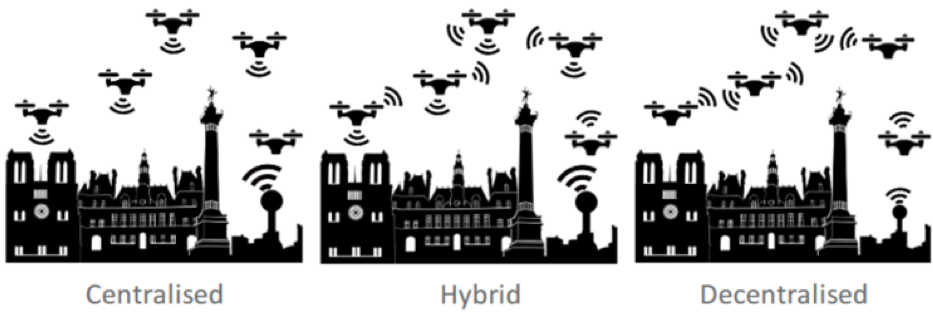
\includegraphics[width=.7\textwidth]{img/metropolis-ii-airspace.png}
    \caption{Metropolis 2: Air traffic control concepts \cite{Badea_2022}.}
    \label{atc-concepts}
\end{figure}

According to Badea \cite{Badea_2022}, the simulations revealed that each concept has trade-offs. 
The centralised model achieved the highest route efficiency but lacked scalability. 
The decentralised model ensured fair access to airspace but struggled with conflict management. 
The hybrid approach provided the best safety performance and balanced traffic distribution, showcasing the benefits of combining proactive (strategic) and reactive (tactical) elements.


\subsubsection{Implications for the Future of AI in ATM}

The findings of Metropolis and Metropolis 2 underscore the vital role that \gls{AI} will play in the future of \gls{ATM}. 
In particular:
\begin{itemize}
    \item \Gls{AI} algorithms such as A*, \gls{MVP}, and conflict resolution heuristics are critical for enabling dynamic, decentralised trajectory planning.
    \item Multi-agent reinforcement learning (MARL) and predictive models could further enhance the hybrid model by learning optimal conflict-avoidance behaviours in real time.
    \item Strategic \gls{AI} planning systems are needed to anticipate demand surges, optimise vertical and horizontal traffic flow, and ensure robust safety margins under uncertainty.
\end{itemize}

% In summary, the future separation management system in high-density urban airspace will likely adopt a hybrid approach powered by \gls{AI}. 
% Such a system would combine centralised strategic optimisation with decentralised, \gls{AI}-driven tactical deconfliction, ensuring both safety and equitable access while adapting to uncertainties in environment, demand, and infrastructure.



% In the first Metropolis project, its aim was to investigate the influence of airspace structure on capacity, complexity, safety, and efficiency for high-density airspace.
% Four airspace concepts, named Full Mix, Layers, Zones, and Tubes, have been defined using increasing levels of structure to implicitly separate and organise traffic.
% Figure \ref{airspace-concepts} shows the visualisation of the four airspace concepts and the following describes the concepts in detail:
% \begin{itemize}
%     \item Full-Mix: `unstructured airspace' where traffic is subjected to only physcal constraints, such as weather, static obstacles and terrain.
%     \item Layers: airspace is segmented into vertically stacked bands, where each altitude layer limits horizontal travel to within allowed heading range
%     \item Zones: segments traffic based layout of the city (current airspace layout).
%     \item Tubes: provides a fixed route structure in the air (allows traffic flow by means of pre-planned conflict free zones).
% \end{itemize}

% \begin{figure}[!ht]
%     \centering
%     \begin{subfigure}{.23\textwidth}
%         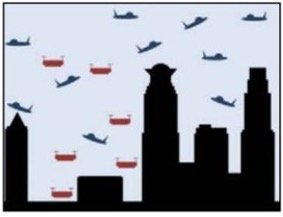
\includegraphics[width=\textwidth]{img/full-mix.jpg}
%         \caption{Full-Mix}
%         \label{full-mix}
%     \end{subfigure}
%     \begin{subfigure}{.23\textwidth}
%         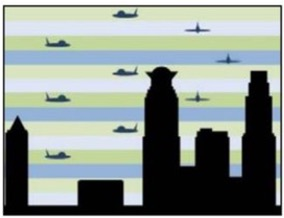
\includegraphics[width=\textwidth]{img/layers.jpg}
%         \caption{Layers}
%         \label{layers}
%     \end{subfigure}
%     \begin{subfigure}{.23\textwidth}
%         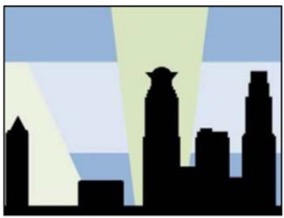
\includegraphics[width=\textwidth]{img/zones.jpg}
%         \caption{Zones}
%         \label{Zones}
%     \end{subfigure}
%     \begin{subfigure}{.23\textwidth}
%         
\includegraphics[width=\textwidth]{img/tubes.jpg}
%         \caption{Tubes}
%         \label{tubes}
%     \end{subfigure}
%     \caption{Metropolis: Airspace concepts \cite{Schuchardt_2023}.}
%     \label{airspace-concepts}
% \end{figure}

% The study by Sunil et al. \cite{Sunil_2015} was done to study if more structuring in the airspace increases the capacity. 
% The aircrafts in Full-Mix, Layers and Zones uses \gls{MVP} algorithm for conflict resolution. 
% Additionally, aircrafts in Zones can select its  altitude flexibly with its horizontal path calculated using A* shortest path algorithm from origin to departure.
% Aircrafts in Tubes plans its route using A* depth-first search algorithm for the shoprtest trajectory from origin to departure prior to departure. 

% Through simulations done in the study, Tubes is not able to meet up the traffic demand, while the others are able to meet the demand. It is also concluded that capacity of airspace also depends on other metrics, such as safety and efficiency.

% The degree of safety of an airspace is assessed by the number of separation violotions.
% Despite the goal of de-conflicting traffic, the resulting high traffic concentrations of the Zones and Tubes concepts apparently has a larger effect than the reduction of relative velocity.

% Both the Full Mix and Layer concepts dstribute traffic over the available airspace, which significantly reduced the number of conflicts and intrusions relative to the more structured concepts.
% Layers concept has the lowest number of intrusions with increasing traffic density.

% Efficiency is defined as the shortest distance between origin and destination, divided by the actual distance travelled.
% Concepts with little structure (i.e. Full Mix and Layers) clearly outperform the highly-structured concepts (Zones and Tubes).

% Through this study, it can be concluded from the comparison of the concepts that for the nominal situtions of a spread demand for \glspl{UAV}, the layered concept is optimal. 




% In the subsequent Metropolis 2 project, it aims to study and develop methodologies to provide \gls{UTM} solution for mixed airspace (open and constrained), which includes airspace design, flight planning, and separation management.
% Despite from the previous Metropolis project showed that the Layered concept is optimal for maximising the airspace, it may not be feasible in cities with very tall buildings (e.g. New York).

% Three concepts wit varying degree of centralisation (Figure \ref{atc-concepts}) will be compared using simulations:
% \begin{itemize}
%     \item Centralised: Focuses on strategic deconfliction and flight planning, which are conducted pre-flight by a central entity. The central entity has access to global data concerning the information of the requested flights, planned flights, and the real-time tracking data of en-route aircrafts.
%     \item Decentralised: Responsible of designing the flight plan and taking the actions to maintain the separation distance lies to each individual agent. The agents do not have any information about the flight plans of other agents and they are not able to include strategic separation techniques while designing their flight plans. 
%     \item Hybrid: Combines centralised and decentralised components to achieve separation management.
% \end{itemize}
% The shortest path from origin to destination for each centralisation model is some variation of A* search algorithm.


% \begin{figure}[!ht]
%     \centering
%     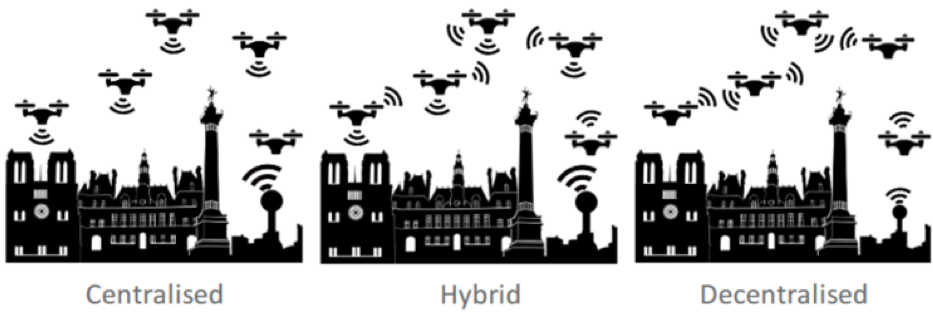
\includegraphics[width=.7\textwidth]{img/metropolis-ii-airspace.png}
%     \caption{Metropolis 2: Air traffic control concepts \cite{Badea_2022}.}
%     \label{atc-concepts}
% \end{figure}

% After the conclusion of the project, it shows that all concepts have strong and weak points, with the hybrid concept excelling in airspace safety, the centralised concept achieving the best overall route efficiency, and the decentralised concept providing the most equitable access to U-space for all operators while also achieving efficiency levels close to the centralised concept.
% Thus, a clear recommendation for the implementation of either of the concepts as designed within the Metropolis 2 cannot be made, as neither achieved an acceptable level of performance in all key performance indicators \cite{Badea_2022}.
% However, a more in-depth analysis of the results reveals that the hybrid use of both central planning and tactical deconfliction has the potential to achieve better results than preponderant use of either.
% The benefits of strategic planning are clear, with traffic being better distributed within the network both in the vertical and horizontal dimensions, which greatly reduces the number of conflicts.
% The implementation of the hybrid concept also showcased that avoiding the congested city center can be a viable strategy for increasing safety at the cost of efficiency. 
% In summary, the future separation management system for urban airspace with high traffic densities will require a combination of proactive and reactive elements, that has the ability to strategically optimise traffic flows, while reactive strategies to ensure equitable use of airspace, and robustness to uncertainties in environment and operations. 

